%\hspace{-1.3mm}[4~v\textsuperscript{o}] habeo suspectam \edtext{falsitatis. Equidem}{\lemma{falsitatis.}\Bfootnote{\textit{(1)} Nam \textit{(2)} Equidem \textit{L}}} supponendo infinitos istos arcus lineis rectis aequales. 
%Sit \edtext{centro H}{\lemma{}\Bfootnote{centro H \textit{erg. L}}} circulus $ABC$ in cujus puncto $E$, sit tangens infinite parva $DE$, et ipsi $AC$ parallela
\noindent  circulus \setline{18}$ABC$ in cujus puncto $E$, sit tangens infinite parva $DE$, et ipsi $AC$ parallela $DF$ ad quam perpendicularis $EF$, et $BG$ \edtext{sinus anguli}{\lemma{}\Bfootnote{sinus \textbar\ versus \textit{gestr.} \textbar\ anguli \textit{L}\hspace{-3mm}}} $AHB$ erunt Triangula $DFE$ et $BGH$ similia adeoque [$DE$]\edtext{}{\Bfootnote{$BE$\textit{\ L \"{a}ndert Hrsg.}\hspace{-3mm}}}, ad $DF$ ut $BH$ ad $BG$. Jam \edtext{tempus ponderis\protect\index{Sachverzeichnis}{pondus} descendentis per $DE$ est aequale tempori}{\lemma{Jam}\Bfootnote{\textit{(1)} celeritas ponderis\protect\index{Sachverzeichnis}{celeritas ponderis} descendentis per $DE$ est \textit{(a)} ad celeritatem \textit{(b)} aequalis celeritati \textit{(2)} tempus [...] tempori \textit{L}\hspace{-3mm}}} ponderis descendentis per $DF$. Spatia autem inaequalia sunt. Ergo \edtext{celeritates\protect\index{Sachverzeichnis}{celeritas} erunt ut spatia percursa\protect\index{Sachverzeichnis}{spatia percursa} reciproce, ergo et vires\protect\index{Sachverzeichnis}{vis}}{\lemma{Ergo}\Bfootnote{\textit{(1)} vires erunt ut spatia \textit{(2)} celeritates [...] vires \textit{L}}}, \edtext{igitur}{\lemma{}\Bfootnote{igitur \textit{erg. L}\hspace{-3mm}}} vis\protect\index{Sachverzeichnis}{vis ponderis} ponderis in circumferentiae circuli puncto $B$, descensum molientis est ad \edtext{vim\protect\index{Sachverzeichnis}{vis} ejusdem [librae] descendentis in}{\lemma{vim}\Bfootnote{\textit{(1)} corporis in \textit{(2)} ejusdem \textbar\ liberi \textit{\"{a}ndert Hrsg.} \textbar\ descendentis in \textit{L}\hspace{-3mm}}} perpendiculari $DF$, ut $DF$ ad $DE$, \edtext{seu ut sinus rectus $BG$ ad radium $BH$}{\lemma{seu ut}\Bfootnote{\textit{(1)} radius $BH$, ad sinum rectum $BG$ \textit{(2)} sinus [...] $BH$ \textit{L}\hspace{-3mm}}}. Eodem modo vis\protect\index{Sachverzeichnis}{vis ponderis} ponderis in \edtext{[$NQ$]}{\lemma{$LD$}\Bfootnote{\textit{L \"{a}ndert Hrsg.}}}
ad vim ponderis in
\edtext{[$LD$]}{\lemma{$NQ$}\Bfootnote{\textit{L \"{a}ndert Hrsg.}}} est ut $PM$ \edtext{ad radium}{\lemma{ad}\Bfootnote{\textit{(1)} sinum \textit{(2)} radium \textit{L}}} $HM$.
\pend 
\pstart
\count\Bfootins=1500
\noindent
\centering
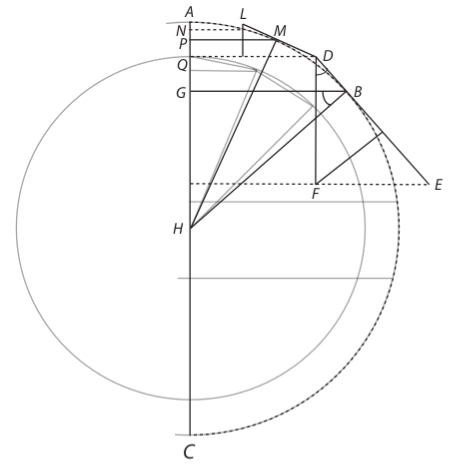
\includegraphics[width=0.65\textwidth]{images/lh0351009_004v-d1.pdf}\\
\centering [\textit{Fig. 6}]
\pend
\pstart \vspace{1em}Jam \setline{1}ponamus pondus descendisse per $LD$, \edtext{quae cum sit infinite parva nullam in ea considerabimus accelerationem\protect\index{Sachverzeichnis}{acceleratio}.}{\lemma{$LD$,}\Bfootnote{\textit{(1)} ducenda erit vis\protect\index{Sachverzeichnis}{vis} \textit{(2)} vis est \textit{(3)} sine acceleratione, ducenda est \textit{(4)} quae [...] accelerationem\protect\index{Sachverzeichnis}{acceleratio}. \textit{L}}} Ponendo radium 1 vis descendentis in $LD$ \edtext{erit $\sqcap \hspace{0.6mm}PM$}{\lemma{erit}\Bfootnote{\textit{(1)} $y\hspace{0.6mm} \sqcap$ \textit{(2)} $\sqcap \hspace{0.6mm}PM$. \textit{L}}}. 
\pend 
\pstart Pone corpus aliquod grave descendere in recta $AF$, ac primum percurrere $AB$ spatium minus quovis dato, \edtext{in tempore minore quovis dato $BC$}{\lemma{dato,}\Bfootnote{\textit{(1)} $\sqcap$ \textit{(2)} in [...] dato $BC$ \textit{L}}} spatium $BD$ \edtext{in tempore $DE$}{\lemma{$BD$}\Bfootnote{\textit{(1)} absolvet \textit{(2)} in tempore $DE$, \textit{L}}}, et spatium $DF$ in tempore \edtext{$FG$, erit tempus}{\lemma{$FG$,}\Bfootnote{\textit{(1)} erunt spatia in \textit{(2)} erit tempus \textit{L}}} quo percurritur spatium $AD$, ad tempus quo percurritur spatium $AF$, ut $ADE$ ad $AFG$, seu in duplicata spatiorum ratione.
Itaque \edtext{si grave per spatium pedis unius}{\lemma{si}\Bfootnote{\textit{(1)} mobile spatium 1 \textit{(2)} grave per spatium pedis unius \textit{L}}} descendet scrupulo secundo unico, descendet per spatium duorum scrupulis secundis quatuor, atque ita retardabitur motus. Jam contra fingamus $AB$ esse vel $AD$ vel $AF$ esse tempus et $BC$, $DE$, $FG$ esse spatium; erunt spatia percursa in duplicata temporum ratione, et per consequens; ita motus accelerabitur. Tempus ergo
\pend
\pstart
%\vspace{1ex}
\noindent
\begin{minipage}[t]{0.5\textwidth}
\hspace*{15mm}
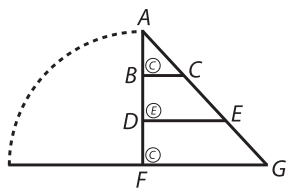
\includegraphics[width=0.75\textwidth]{images/lh0351009_004v-d2.pdf}
%\noindent \centering [\textit{Fig. 7}]
\end{minipage}
\hspace*{25mm}
\begin{minipage}[t]{0.5\textwidth}
%\hspace*{-5mm}
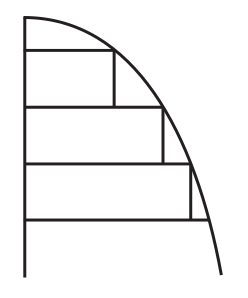
\includegraphics[width=0.45\textwidth]{images/lh0351009_004v-d2a.pdf}
%\noindent \centering [\textit{Fig. 8}]
\end{minipage}\\
\vspace{8mm}
\hspace*{32mm} [\textit{Fig. 7}] \hspace*{55mm}  [\textit{Fig. 8}]
\pend
%\vspace{0.5em}
\vspace{1.5em}
\pstart
\noindent
\begin{minipage}[t]{0.5\textwidth}
\hspace*{23mm}                    
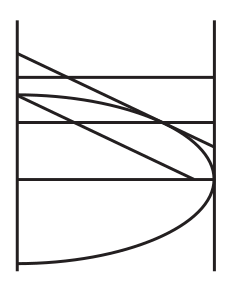
\includegraphics[width=0.45\textwidth]{images/lh0351009_004v-d3.pdf}
\end{minipage}
\hspace*{25mm}
\begin{minipage}[t]{0.5\textwidth}
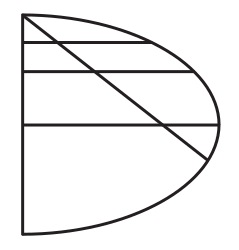
\includegraphics[width=0.45\textwidth]{images/lh0351009_004v-d4.pdf}
% [\textit{Fig. 9}] \hspace{15mm} [\textit{Fig. 10}]
\end{minipage}\\
\vspace{8mm}
\hspace*{32mm} [\textit{Fig. 9}] \hspace*{55mm}  [\textit{Fig. 10}]\setline{1}
\pend
\vspace{2.5em}
\pstart \noindent considerandum \setline{1}est velut partes axis; vis simplex\protect\index{Sachverzeichnis}{vis simplex} in quolibet momento temporis exercita velut differentiae ordinatarum; vis acquisita\protect\index{Sachverzeichnis}{vis acquisita} in quolibet momento temporis, velut ordinatae; vires\protect\index{Sachverzeichnis}{vis} inter se ut ordinatae figurae: spatia percursa ut \edtext{portiones figurae}{\lemma{ut}\Bfootnote{\textit{(1)} spatia \textit{(2)} portiones figurae \textit{L}}}. Figura autem est semper Quadratrix \edtext{figurae differentiarum}{\lemma{Quadratrix}\Bfootnote{\textit{(1)} ordinatarum \textit{(2)} figurae differentiarum \textit{L}}} seu virium simplicium\protect\index{Sachverzeichnis}{vis simplex}.
\pend 
\vspace{2mm}
\count\Afootins=1250
\count\Cfootins=1250
%\newpage
\pstart \noindent$y + \sqrt{a^2 - y^2} \sqcap x.$ maximo. \\
\rule[-4mm]{0mm}{10mm}$ a^2 \raisebox{-3.2mm}{{\def\firstcircle{(0,0) circle (0.4cm)}\begin{tikzpicture}\draw \firstcircle node {$-y^2$};\end{tikzpicture}}} \sqcap x^2 - 2yx \raisebox{-3.2mm}{{\def\firstcircle{(0,0) circle (0.4cm)}\begin{tikzpicture}\draw \firstcircle node {$+y^2$};\end{tikzpicture}}}$\\
\rule[0pt]{26mm}{0pt} $+2y^2$\\
$-x^2 + 2yx \cdot \cdot\ + 2y^2 - 2yx$\\
$-\cancel{2}x^2 + \cancel{2}yx \sqcap + \overset{2}{\cancel4}yl - \cancel{2}lx$\\
\rule[-4mm]{0pt}{10mm}$l \sqcap \displaystyle\frac{-2x^2 + 2yx}{+2y - x}$\edtext{}{\lemma{$l \sqcap \displaystyle\frac{-2x^2 + 2yx}{+2y - x}$}\Cfootnote{Die Division durch 2 wurde nur im Nenner berücksichtigt. Der Fehler wirkt sich auf die weitere Ableitung aus.}}\\
\rule[-4mm]{0pt}{10mm}$x^2 \sqcap \raisebox{-3.2mm}{{\def\firstcircle{(0,0) circle (0.4cm)}\begin{tikzpicture}\draw \firstcircle node {$y^2$};\end{tikzpicture}}} + 2\sqrt{a^2 - y^2} + a^2 \raisebox{-3.2mm}{{\def\firstcircle{(0,0) circle (0.4cm)}\begin{tikzpicture}\draw \firstcircle node {$-y^2$};\end{tikzpicture}}}$\edtext{}{\lemma{$2\sqrt{a^2-y^2}$}\Cfootnote{Der Term lautet eigentlich
 $2y\sqrt{a^2-y^2}$. Der Fehler wirkt sich auf die weitere Ableitung aus.}}\\
\rule[-4mm]{0pt}{10mm}$l \sqcap \displaystyle\frac{-4\sqrt{a^2 - y^2} - 2a^2 + 2y^2 + 2y\sqrt{a^2 - y^2}}{\raisebox{-3.2mm}{{\def\firstcircle{(0,0) circle (0.4cm)}\begin{tikzpicture}\draw \firstcircle node {$2$};\end{tikzpicture}}} \ y \ \raisebox{-3.2mm}{{\def\firstcircle{(0,0) circle (0.4cm)}\begin{tikzpicture}\draw \firstcircle node {$-y$};\end{tikzpicture}}} - \sqrt{a^2 - y^2}}$\edtext{}{\lemma{$-4\sqrt{a^2 - y^2} - 2a^2 + 2y^2 + 2y\sqrt{a^2 - y^2}$}\Cfootnote{Der Z\"{a}hler lautet eigentlich
 $-2y\sqrt{a^2 - y^2} - a^2 + y^2 + y\sqrt{a^2 - y^2}$.}}\\
\rule[-4mm]{0pt}{10mm}$y \sqcap \sqrt{a^2 - y^2}$\hspace{3mm} $y^2 \sqcap a^2 - y^2$. Ergo $2y^2 \sqcap a^2$. Ergo $y \sqcap \displaystyle\frac{\PsMs\hspace{0.4mm} a}{\sqrt 2} \quad\displaystyle\frac{a}{1\displaystyle\frac{2}{5}} \quad \begin{array}{cc}a\\
\hline\hline \displaystyle\frac{7}{5} \end{array} \quad\displaystyle\frac{5a}{7}.$\edtext{}{\lemma{}\Afootnote{\textit{Nebenrechnungen}:\\ $\displaystyle\frac{200}{100}$ \hspace{3mm} $\displaystyle\frac{\displaystyle\efrac{\cancel{1}\cancel{2} 4}{\text{\d{$\cancel{\bullet}$}}\cancel{\bullet}\text{\d{$\cancel{\bullet}$}}}}{\displaystyle\frac{1\,\,\,4}{\cancel{1}\cancel{2}\cancel{4}}}$ \hspace{3mm} $\displaystyle\frac{14}{10} \bigg\vert \displaystyle\frac{7}{5} \sqcap 1 \displaystyle\frac{2}{5}$\vspace{-4mm}}}\\
$2y \sqcap x. \quad 2y \sqcap y + \sqrt{a^2 - y^2},$ ou $y \sqcap \sqrt{a^2 - y^2}$ ou $y^2 \sqcap a^2 - y^2$ ou $2y^2 \sqcap a^2.$ \edlabel{vismach1}
\edtext{}{{\xxref{vismach1}{vismach2}}\lemma{$y \hspace{0.3mm}\sqcap \displaystyle\frac{a}{\sqrt2}$}\Bfootnote{\textit{(1)} $z + \sqrt{2az - z^2}\hspace{0.4mm} \sqcap \hspace{0.4mm}\omega$ \hspace{1mm}  $\omega^2 - 2 \omega z + \cancel{2}z^2 \hspace{0.4mm}\sqcap \hspace{0.4mm}2az \protect\ovalbox{$-z^2$}$.\hspace{0.2mm} $\protect\begin{array}{ll}\cancel{2}\omega^2 - \cancel{2}\omega z + \cdots \sqcap - \protect\overset{2}{\cancel4}z^{\protect\textcircled{$\scriptstyle 2$}}\lambda &+\cancel{2}\omega \protect\textcircled{z} \lambda.\\ &+\cancel{2}a \,\,\cdot \;\;\cdot\protect\end{array}$ 
$\protect\begin{array}{rl}\hspace{-1.8mm}\lambda \sqcap \displaystyle\frac{\omega^2 - \omega z}{-2z + \omega} & \protect\atop{}{\displaystyle{2z \sqcap \omega + a. \quad z \sqcap \omega + a.}}\\ +a & \ \ z\sqcap z - \protect\end{array}$ \textit{ (2) } $a-z + \sqrt{2az - z^2} \sqcap \omega.$ Ergo [...] $\lambda \sqcap \displaystyle\frac{\displaystyle\efrac{\omega^2 +z \omega}{\quad \quad -a \cdot \cdot}}{\displaystyle\efrac{-2z + 2a}{\quad \quad\, - \omega}}$ \textit{ L}}} 
$y \sqcap \displaystyle\frac{a}{\sqrt2}$\\
\rule[-4mm]{0pt}{10mm}$a-z + \sqrt{2az - z^2} \sqcap \omega.$ Ergo  $2az - z^2 \sqcap \omega + z - a, \Box\\ 
\!\sqcap \,\omega^2 + 2\omega z - 2\omega a, + z^2 - 2az + a^2$. \rule[-4mm]{0pt}{10mm}Ergo 
\pend 
\newpage
\count\Afootins=1500
\count\Cfootins=1500
\vspace{1ex} 
\pstart\noindent
%yellow
$\begin{array}{lll}-\overset{2}{\cancel4} z^2 & + \overset{2}{\cancel4}a\text{\td{\textit{z}}} \cdot \cdot \cdot \cdot \cancel{2}\omega^2 & + \cancel{2}z\text{\td{\textit{\pgrk{w}}}}.\\ & -\cancel2 \omega & - \cancel{2}a \end{array}$\\ \vspace{0.5ex} $\lambda \sqcap \displaystyle\frac{\displaystyle\efrac{\omega^2 +z \omega}{\quad -a \cdot \cdot}}{\displaystyle\efrac{-2z + 2a}{\quad\, - \omega}}$\edlabel{vismach2}
%\edtext{}{{\xxref{vismach1}{vismach2}}\lemma{$y \hspace{0.3mm}\sqcap \displaystyle\frac{a}{\sqrt2}$}\Bfootnote{\textit{(1)} $z + \sqrt{2az - z^2}\hspace{0.4mm} \sqcap \hspace{0.4mm}\omega$ \hspace{3mm}  $\omega^2 - 2 \omega z + \cancel{2}z^2 \hspace{0.4mm}\sqcap \hspace{0.4mm}2az \protect\ovalbox{$-z^2$}$.\hspace{3mm} $\protect\begin{array}{ll}\cancel{2}\omega^2 - \cancel{2}\omega z + \cdots \sqcap - \protect\overset{2}{\cancel4}z^{\protect\textcircled{$\scriptstyle 2$}}\lambda &+\cancel{2}\omega \protect\textcircled{z} \lambda.\\ &+\cancel{2}a \,\,\cdot \;\;\cdot\protect\end{array}$ \hspace{3mm} $\protect\begin{array}{rl}\lambda \sqcap \displaystyle\frac{\omega^2 - \omega z}{-2z + \omega} & \protect\atop{}{\displaystyle{2z \sqcap \omega + a. \quad z \sqcap \omega + a.}}\\ +a & \ \ z\sqcap z - \protect\end{array}$ \textit{ (2) } $a-z + \sqrt{2az - z^2} \sqcap \omega.$ Ergo [...] $\lambda \sqcap \displaystyle\frac{\displaystyle\efrac{\omega^2 +z \omega}{\quad \quad -a \cdot \cdot}}{\displaystyle\efrac{-2z + 2a}{\quad \quad\, - \omega}}$ \textit{ L}}} 
$ \quad 
%
% BEGIN NEW
% Der Befehl \crossedcircle{x} erzeugt einen Kreis, der unten links zweimal durchgestrichen ist. 
% Das Argument x erscheint innerhalb des Kreises.
% Achtung: Das funktioniert nur mit einem Argument, das aus einem einzigen Zeichen, z.B. 2 oder a, besteht.
\efrac{\displaystyle \raisebox{-1.2mm}{{\def\firstcircle{(0,0) circle (0.2cm)}\begin{tikzpicture}\draw \firstcircle node {$2$};\end{tikzpicture}}}
\,z + \omega \sqcap \crossedcircle{2} \, a \cdot \cdot}
{\displaystyle\overbrace{\crossedcircle{a}\raisebox{-1.2mm}{{\def\firstcircle{(0,0) circle (0.25cm)}\begin{tikzpicture}\draw \firstcircle node {$-z$};\end{tikzpicture}}} + \sqrt{2az - z^2}}}
% END NEW
%
\quad z + \sqrt{2az - z^2}\sqcap a \quad 2az - z^2 \sqcap a^2 - 2az + z^2$
\pend
%\newpage
\pstart \noindent $2z^2 - 2az - a^2 \sqcap 0$\edtext{}{\lemma{$2z^2 - 2az - a^2 \sqcap 0$}\Cfootnote{Die Gleichung lautet eigentlich
 $2z^2  -4az + a^2 \sqcap 0$. Der Fehler wirkt sich bis zum Ende der Rechnung aus.}} $\quad z^2 - az + \displaystyle\frac{a^2}{4} \sqcap \ovalbox{$\displaystyle\frac{a^2}{2} + \displaystyle\frac{a^2}{4}$} \,\displaystyle\frac{3}{4}a^2 \quad \PsMs \hspace{0.4mm}z \hspace{0.4mm}\MsPs \hspace{0.4mm}\displaystyle\frac{a}{2} \sqcap \displaystyle\frac{a\sqrt3}{2}\cdot \quad z \sqcap \displaystyle\frac{\PsMs \hspace{0.4mm}a\sqrt3 + a}{2}$\\
$2az - z^2 \sqcap y^2 \quad \ovalbox{$\PsMs \hspace{0.4mm}2a^2 \sqrt3$} + 2a^2 - 3a^2 \ovalbox{$\MsPs \hspace{0.4mm}2a^2 \sqrt3$} - a^2 \sqcap z^2 - \displaystyle\frac{a^2}{2} - a^2 \quad \ovalbox{$-2az + z^2$} \sqcap \displaystyle\frac{-a^2}{2}$\rule[-4mm]{0pt}{10mm}\\
%\pend
%\newpage
%\pstart\noindent
%orange
\rule[-4mm]{0pt}{10mm}$2z^2 - 2az\setline{5} \sqcap a^2$, sive $z^2 + $ \raisebox{-2ex}{$\displaystyle\efrac{\underbrace{z^2 - 2az}}{-y^2 \sqcap - \displaystyle\frac{a^2}{2}}$} $\sqcap \hspace{1mm}a^2.$ Ergo $z \sqcap \displaystyle\frac{a \sqrt3}{2}$ et $z^2 \sqcap \displaystyle\frac{3a^2}{4}$ \edtext{et $2az - z^2 \sqcap \edlabel{LH0351009_004v_aa}2a^2 \sqrt3\edlabel{LH0351009_004v_bb} - \displaystyle\frac{3a^2}{4} \sqcap \displaystyle\frac{a^2}{2}.$}{\lemma{et}\Bfootnote{\textit{ (1) } $z^2 - 2az$ \textit{ (2) } $2az - z^2 \sqcap 2a^2 \sqrt3 - \displaystyle\frac{3a^2}{4} \sqcap \displaystyle\frac{a^2}{2}.$ \textit{ L}}}
\edtext{}{{\xxref{LH0351009_004v_aa}{LH0351009_004v_bb}}{\lemma{$2a^2 \sqrt3$}\Cfootnote{Richtig heißt es $a^2 \sqrt3$.
Der Fehler wirkt sich bis zum Ende der Rechnung aus.}}} \rule[-4mm]{0mm}{10mm}Ergo $8a^2 \sqrt3 - 3a^2 \sqcap 2a^2 \quad 8a^2 \sqrt3 \sqcap 5a^2$ \hspace{2em} $8\sqrt3 \sqcap 5.$ \hspace{2em} $64 \smallfrown 3 \sqcap 25$ absurdum. Error. 
\pend  